\documentclass[logo,reportComp]{thesis}
\usepackage[cpp,pseudo]{mypackage}

\title{高级编程技术实验报告}
\subtitle{实验三:Word Game}
\school{数据科学与计算机学院}
\author{陈鸿峥}
\classname{17大数据与人工智能}
\stunum{17341015}
\headercontext{高级编程技术实验报告}
% \authorremark{本实验报告用\LaTeX撰写,创建时间:\builddate\today}

\begin{document}

\maketitle

\section{问题描述及求解思路}
实现一个单词游戏(word game)。
每轮游戏会发给玩家几张字母牌,通过组合字母牌上的字母组合出单词。

\subsection{单词分数}
\verb'get_word_score'将单词\verb'word'转为小写后,遍历其中的每一个字母,并在\verb'SCRABBLE_LETTER_VALUES'中获取该字母的分数。
将分数累加即得该单词的得分。

\subsection{处理手牌}
\verb'update_hand'用于出了一次完整单词后更新手牌内容及数目。
将遍历打出的单词\verb'word'中的每一个字母,通过\verb'get'函数获得其是否在手牌中出现,以避免出现错误情况(即0张手牌但没有从字典中清除的情况)。
如果出现,则对该字母对应的手牌数减1。

\subsection{单词合法性}
\verb'is_valid_word'先将\verb'word'中的字母全部转为小写,然后遍历\verb'word_list',判断该小写单词是否在单词表中。
另外,还需用类似\verb'update_hand'的方法判断\verb'word'中的字母是否全部由原有的手牌构成。

\subsection{通配符}
注意通配符(wildcard)只能替代元音字母。

\verb'is_valid_word'中添加通配符的判断:如果存在通配符,则遍历所有元音字母,并替换掉通配符,尝试匹配单词表\verb'word_list'中的单词。
若对于所有元音字母替换,都找不到对应的单词,则说明\verb'word'不是一个合法的单词。
如果没有通配符,则代码实现逻辑与上题相同。

\verb'deal_hand'按照题目叙述的方式进行实施,减少一个元音位置,留给通配符使用。
注意要在程序引言区添加\verb'WILDCARD'变量。
处理\verb'hand'时同样用了\verb'get'方法字典匹配不成功报错。

\subsection{出牌实施}
游戏规则见题目要求,在此不再赘述。

\verb'play_hand'函数具体实施如下
\begin{enumerate}
	\item 初始化分数计数器\verb'total_score'为0
	\item 当手上还有牌时,进入\verb'while'循环
	\item 用\verb'display_hand'展示当前手牌
	\item 请求用户输入,如果输入为\verb'!!'则结束游戏,否则继续进行
	\item 用\verb'is_valid_word'判断用户单词是否合法,如果合法则得分\verb'get_word_score',否则输出错误提示信息
	\item 用\verb'update_hand'更新手牌,回到2(注意即使不合法的单词也会消耗手牌!)
	\item 如果手上没牌或得到\verb'!!'输入,则游戏结束
	\item 输出用户最终得分
\end{enumerate}

\subsection{完整游戏实施}
\verb'substitute_hand'用于替换手牌,方法与生成手牌的方法类似,即利用\verb'random.choice'方法随机生成。
然后将新生成的手牌结如其中,将原指定手牌丢弃。
注意是替换字母,而不是替换单一手牌,即如果一个字母对应的手牌有多张,则需要全部替换。

\verb'play_game'的实施如下
\begin{itemize}
	\item 用户输入玩牌轮数\verb'n_hands'
	\item 在每一手牌开始之前询问用户是否需要替换手牌,如果需要则询问需要替换哪一张牌,且此操作只能被使用一次,用\verb'flag_sub'记录。
	\item 每一轮手牌结束之后询问用户是否回放上一轮的手牌,如果回放则不给予用户新的手牌。该操作只能用一次,用\verb'flag_replay'记录,但不计入用户的玩牌轮数,且不再拥有替换牌的权利。
\end{itemize}

\section{代码}
代码实施及注释请见附件\verb'ps3.py'。

\section{运行截图}
实验运行结果如下面几幅图片所示,且\textbf{测试了不同样例,以针对不同分支},确保结果的正确性和鲁棒性。
\begin{figure}[H]
\centering
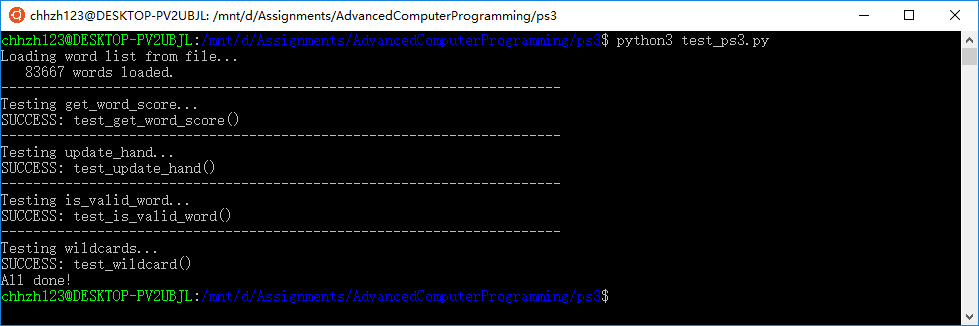
\includegraphics[width=\linewidth]{fig/test-done.PNG}
\caption{测试样例全部通过}
\end{figure}
\begin{figure}[H]
\centering
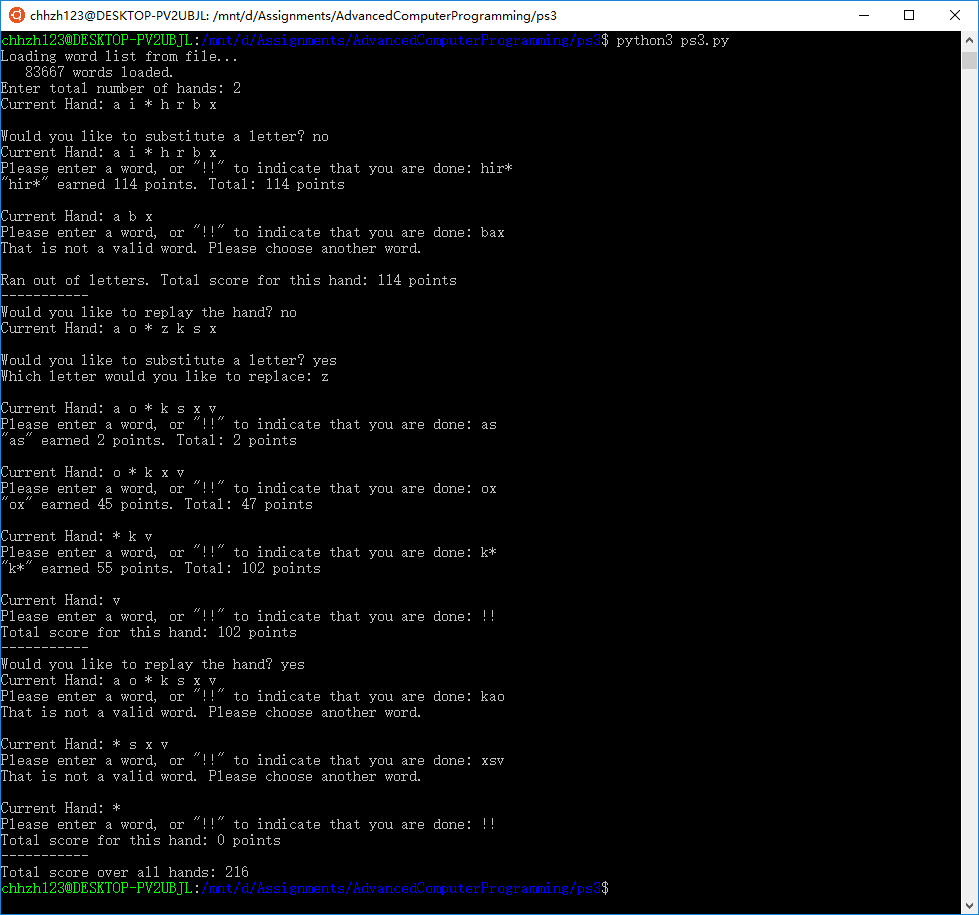
\includegraphics[width=\linewidth]{fig/game.PNG}
\caption{完整游戏}
\end{figure}
\begin{figure}[H]
\centering
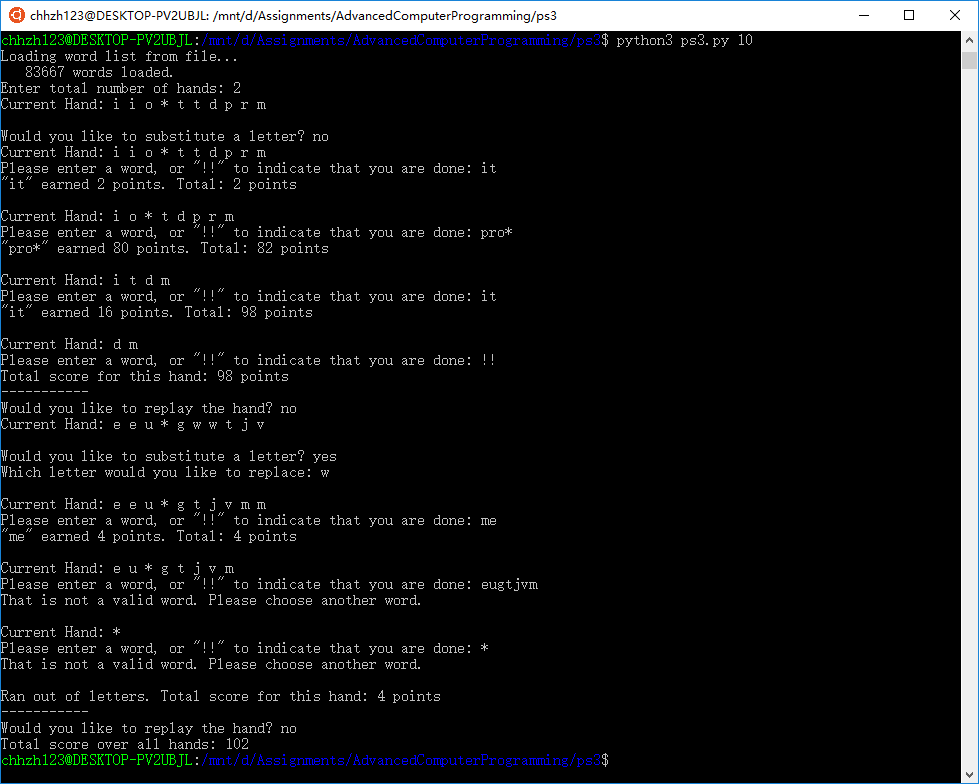
\includegraphics[width=\linewidth]{fig/game-10.PNG}
\caption{自己添加:通过命令行传递参数指明手牌数目,如此图中传递的是10}
\end{figure}

\end{document}

% 实验提交内容
% 邮件主题,作业文件命名规范(学号、姓名)
% 文档pdf格式(问题、求解思路、代码、注释、运行截图)
% 考虑健壮性、可读性
% 极端样例